
%(BEGIN_QUESTION)
% Copyright 2006, Tony R. Kuphaldt, released under the Creative Commons Attribution License (v 1.0)
% This means you may do almost anything with this work of mine, so long as you give me proper credit

Three different forms of globe valve are shown here: {\it stem-guided}, {\it port-guided}, and {\it cage-guided}:

$$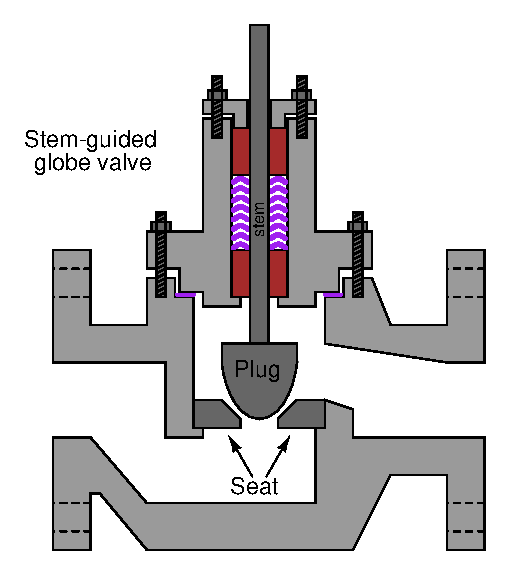
\includegraphics[width=15.5cm]{i00775x01.eps}$$

$$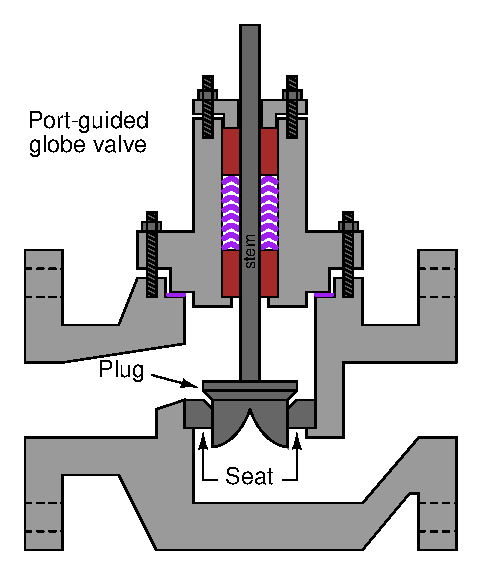
\includegraphics[width=15.5cm]{i00775x02.eps}$$

$$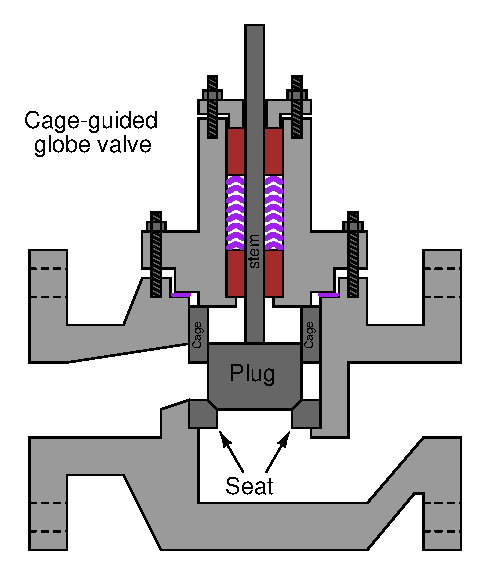
\includegraphics[width=15.5cm]{i00775x03.eps}$$

Describe the differences between these three globe valve designs, and identify which one is more popular in industry today.

\underbar{file i00775}
%(END_QUESTION)





%(BEGIN_ANSWER)

The cage-guided valve design is the most popular today.

\vskip 10pt

In a cage valve, the flow is throttled not by the size of the restriction formed between a contoured plug and the seat, but rather by the restriction formed by the piston-shaped plug's uncovering of holes in the cage.  The seat serves only one purpose, and that is tight shutoff at the 0\% open (fully-closed) position.

Because of this, the seat in a cage valve is subject to less wear than in a globe valve with a contoured plug or a ``v-ported'' plug, extending its service life.  Opening characteristics of the valve (quick-opening, linear, and equal-percentage) may be easily altered by changing only the cage.  In a regular globe valve, the plug must be changed for one of a different contour.  Since cages are more easily changed than plugs, this provides better flexibility.

%(END_ANSWER)





%(BEGIN_NOTES)


%INDEX% Final Control Elements, valve: guiding for globe valves (stem, port, and cage)

%(END_NOTES)


